\documentclass[border=6pt]{standalone}
% Shared preamble for web figures.  Each figure is a standalone .tex that
% \input's this file; scripts/make-figures.sh turns it into an SVG.
% Handouts pull the same file with \fig{Unit_X/<name>}.
\usepackage[T1]{fontenc}
\usepackage{helvet}
\renewcommand{\familydefault}{\sfdefault}
\renewcommand{\ttdefault}{pcr}  % Courier: a real Type 1 typewriter font
\usepackage{amsmath}
\usepackage{tikz}
\usetikzlibrary{arrows.meta,positioning,calc,shapes.symbols,shapes.geometric}

% Who makes the rules is the point of most diagrams in this book, so the
% colors mean the same thing everywhere: blue is a person, orange is the
% computer, green is an answer, pink is the human brain.
\definecolor{person}{HTML}{2C6FAE}
\definecolor{machine}{HTML}{D35400}
\definecolor{result}{HTML}{1E8449}
\definecolor{brainpink}{HTML}{C2185B}
\definecolor{ink}{HTML}{2C3E50}

\tikzset{
  doodle/.style={line width=1.5pt, line cap=round, line join=round, draw=ink},
  box/.style={draw, rounded corners=5pt, line width=1.1pt, align=center,
              inner sep=7pt, minimum height=1.0cm, font=\small},
  personbox/.style={box, draw=person, fill=person!10},
  machinebox/.style={box, draw=machine, fill=machine!10},
  resultbox/.style={box, draw=result, fill=result!10},
  plainbox/.style={box, draw=ink!70, fill=ink!4},
  flow/.style={-{Stealth[length=8pt]}, line width=1.4pt, draw=ink},
}

% A person (blue) and a robot head (orange) as small icons.
% \personicon{x}{y}{scale}   \roboticon{x}{y}{scale}
\newcommand{\personicon}[3]{%
  \begin{scope}[shift={(#1,#2)}, scale=#3]
    \fill[person] (0,0.62) circle (0.28);
    \fill[person, rounded corners=6pt] (-0.42,-0.55) rectangle (0.42,0.28);
  \end{scope}}
\newcommand{\roboticon}[3]{%
  \begin{scope}[shift={(#1,#2)}, scale=#3]
    \draw[machine, line width=1.2pt] (0,0.5) -- (0,0.72);
    \fill[machine] (0,0.78) circle (0.08);
    \draw[machine, line width=1.4pt, fill=machine!12, rounded corners=4pt] (-0.5,-0.45) rectangle (0.5,0.5);
    \fill[ink] (-0.2,0.12) circle (0.08);
    \fill[ink] (0.2,0.12) circle (0.08);
    \draw[ink, line width=1pt] (-0.22,-0.22) -- (0.22,-0.22);
  \end{scope}}

\begin{document}
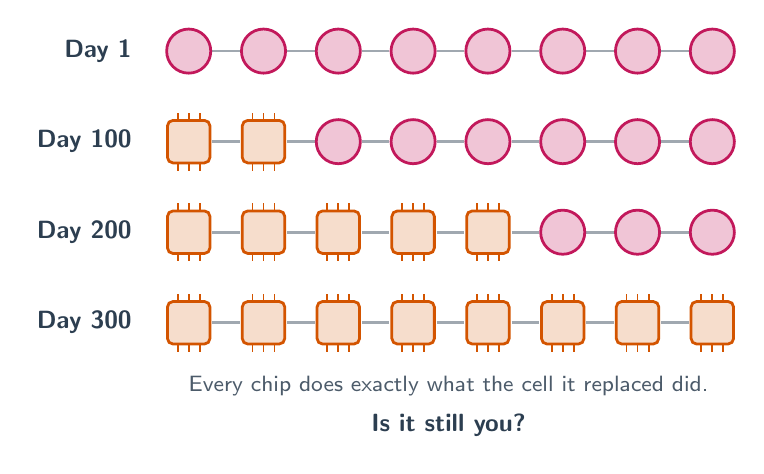
\begin{tikzpicture}[
  lbl/.style={font=\small\bfseries, text=ink, anchor=east},
  sub/.style={font=\footnotesize, text=ink!85, align=center},
]
% Replace a brain one neuron at a time. Pink: a brain cell. Orange: a chip that does the same job.
\newcommand{\cell}[3]{% x, y, kind (0 = neuron, 1 = chip)
  \ifnum#3=0 \fill[brainpink!25, draw=brainpink, line width=1pt] (#1,#2) circle (0.28);
  \else \draw[machine, fill=machine!20, line width=1pt, rounded corners=2pt] (#1-0.27,#2-0.27) rectangle (#1+0.27,#2+0.27);
    \foreach \d in {-0.14,0,0.14} {\draw[machine, line width=0.7pt] (#1+\d,#2+0.27) -- (#1+\d,#2+0.37); \draw[machine, line width=0.7pt] (#1+\d,#2-0.27) -- (#1+\d,#2-0.37);}
  \fi}
\foreach \row/\n/\name in {0/0/Day 1, 1/2/Day 100, 2/5/Day 200, 3/8/Day 300} {
  \pgfmathsetmacro{\y}{-\row*1.15}
  \node[lbl] at (-0.6,\y) {\name};
  \foreach \i in {1,...,8} {
    \pgfmathtruncatemacro{\k}{\i <= \n ? 1 : 0}
    \pgfmathsetmacro{\x}{(\i-1)*0.95}
    \ifnum\i<8 \draw[ink!45, line width=1pt] (\x+0.3,\y) -- (\x+0.65,\y); \fi
    \cell{\x}{\y}{\k}
  }
}
\node[sub] at (3.3,-4.25) {Every chip does exactly what the cell it replaced did.};
\node[sub, font=\small\bfseries, text=ink] at (3.3,-4.75) {Is it still you?};
\end{tikzpicture}
\end{document}
